\documentclass[11pt, a4paper]{article}

\usepackage{amsmath}
\usepackage{amsfonts} %Matheschriften
\usepackage{amssymb} %Mathesymbole
%\usepackage{mathptmx} % Einstellung für Schriften und Sonderzeichen in mathematischen Umgebungen
                        % ändert SChriftfont
\usepackage{wasysym} % Stellt diverse Sonderzeichen bereit
\usepackage{siunitx}
\usepackage{float}
\usepackage{microtype}
\usepackage{graphicx}
\usepackage{hyperref}
\usepackage{xcolor}
\usepackage[section]{placeins}


\usepackage[ngerman]{babel}
\addto\captionsngerman{%
 \renewcommand{\abstractname}{Einleitung}}

\title{Versuch 3: Schiefe Ebene}
\author{Jascha Fricker, Benedict Brouwer}

\begin{document}
    \maketitle

    

    \begin{abstract}
        Schon Gallileo hat mit schiefen Ebenen experiemtiert und auch heute ist die schiefe Ebene ein viel benutztes
        Modell. Auch in diese Versuch betrachten wir eine schiefe Ebene, messen die Kraftkomponenten und
        die Reibung. 
    \end{abstract}

    \tableofcontents

    \newpage

    \section{Kräftezerlegung}
    \subsection{Theorie \& Experimenteller Aufbau}
    Bei einer schiefen Ebene zerlegt sich die wirkende Gravitationskraft in zwei Teilkräfte.
    \begin{align}
        \text{ Normalkraft } \ \ F_\perp = F_g cos \alpha \\
        \text{ Tangentialkraft } \ \ F_\parallel = F_g sin \alpha 
    \end{align}
    Im Experiment werden diese Kräfte mit zwei Kraftmessern für unterschiedliche Winke $\alpha$ bestimmt.

    \subsection{Ergebnisse \& Diskussion}
    \begin{figure}
        \centering
        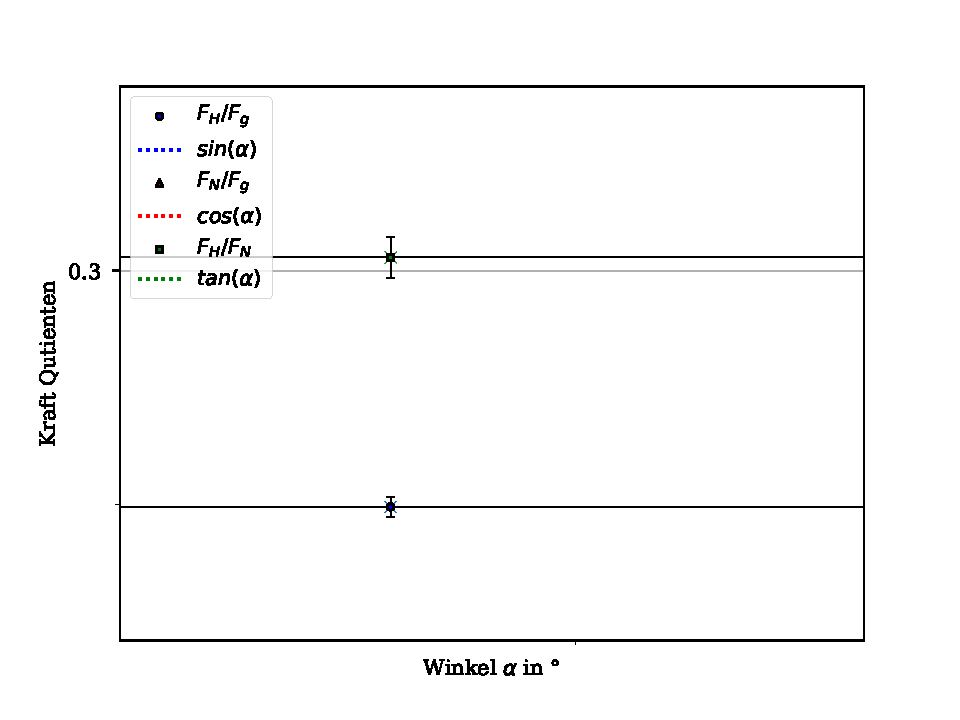
\includegraphics[width=\textwidth]{./5Kraftzer.pdf}

        \caption{Kraftquotienten der Kräftezerlegung}
        \label{fig:Kraftzer}
    \end{figure}
    Im Graph \ref{fig:Kraftzer} sind die die berechneten Kraftquotienten bezüglich der verschiedenen Winkel aufgetragen.
    Es kann erkannt werden, dass die Messwerte sehr stark von den Theoriekurven abweichen, dies liegt wahrscheinlich
    am ungenauen Versuchsaufbau.
    
    In diesem Versuch wurden die Unsicherheiten des Kraftmessers(Schrittweite), die Unsicherheit der Waage($1\si{\gram}$)
    sowie die Unsicherheiten der Winkelmessung(Schrittweite $1 \si{\milli\metre}$) berücksichtigt.
    Durch den Versuchsaufbau konnte nicht verifiziert werden, dass die Normalkraft genau senkrecht anliegt.
    Anhand der Daten lässt sich ein Unsicherheitintervall von etwa $3,5^{\circ}$ ableiten, welches auch zu
    Beobachtungen bei der Versuchsdurchführung passt. Für die Unsicherheiten wurde erst der Mittelwert \cite[(29)]{ABW}
    und die Standardabweichung mithilfe der Student-t-Verteilung \cite[(15)]{ABW} der beiden Kräfte berechnet, um dann mithilfe der Gausschen
    Gausschen Fehlerfortpflanzung \cite[(19)]{ABW} die Unsicherheit der Quotienen zu berechnen.

    \section{Haftreibung}
    \subsection{Theorie \& Experiemteller Aufbau}
    Die Haftreibung ist die Reibungskraft, die existiert, wenn ein Körper sich nicht bewegt.
    Die Haftreibungskraft
    \begin{align}
        F_H = \mu_H \cdot F_n
    \end{align}
    ist proportional zur Normalkraft und zur Haftreibungskonstante $\mu_H$. Um diese zu messen,
    wird mit einem Kraftmesser tangential Kraft an die Masse angelegt. Diese wird langsam erhöht.
    Sobald die Masse anfängt zu rutschen, wird die direkt vorher angelegt Kraft als Haftreibungskraft notiert.

    \subsection{Ergebnis \& Diskussion}
    \begin{figure}
        \centering
        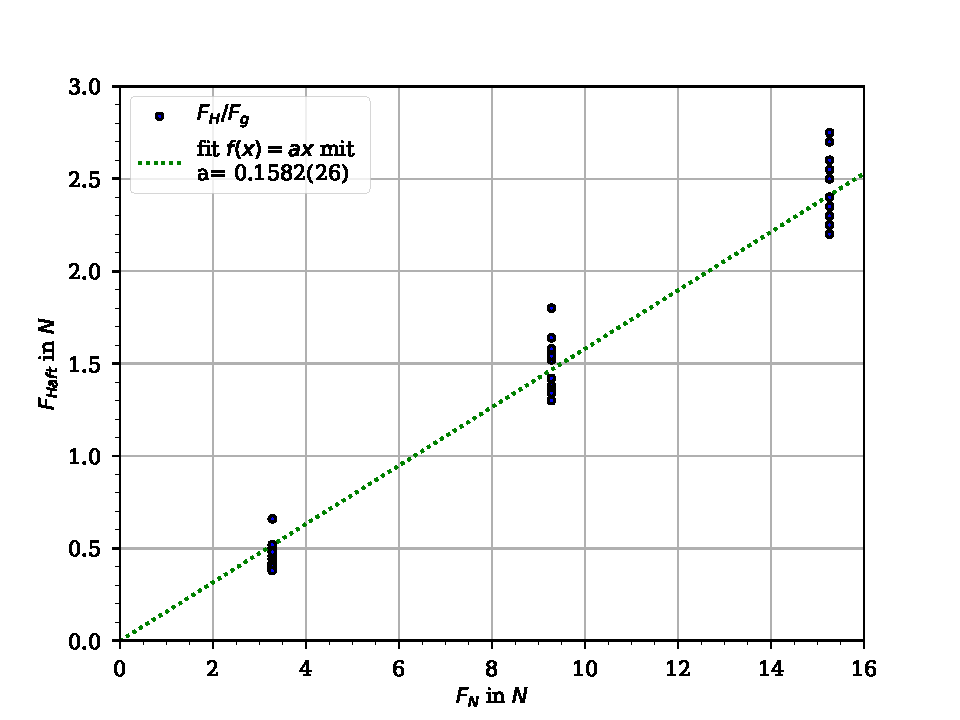
\includegraphics[width=\textwidth]{./6Haftreibc.pdf}

        \caption{Messung der Reibungskraft}
        \label{fig:haftr}
    \end{figure}
    In Graph \ref{fig:haftr} kann anhand der Steigung der Ursprungsgeraden der Haftreibungskoeffizient
    \begin{align}
        \mu_H = 0,1582(26)
    \end{align} 
    bestimmt werden.
    Die große Abweichung der einzelnen Messungen liegt wahrscheinlich an der Inhomogenität der Haftreibung
    abhängig vom Ort, an dem gemessen wurde. Auch beim 3. Versuch haben wir diesen Effekt
    bei der Gleitreibung bei kleinen Winkeln bemerkt. Der Fehler wurde durch das fitten der Gerade
    an alle Messwerte berechnet. Durch die große Anzahl an Messungen konnte die Unsicherheit eines einzelnen
    Fehlers vernachlässigt werden.

    \section{Gleitreibung}

    \subsection{Theorie \& Experimenteller Aufbau}

    Die Gleitreibung ist, im Gegensatz zur Haftreibung, die Reibung, die entsteht, während der Körper gleitet.
    Wenn ein Körper eine schiefe Ebene hinuntergleitet, hat er folgende Bewegungsgleichung:
    \begin{align}
        \text{ohne Reibung:} \ \  s(t) &= \frac{g \cdot sin(\alpha)}{2} \cdot t^2 +v_0 \cdot t + x_0 \\
        \text{mit Reibung:} \ \  s(t) &= g \cdot \frac{sin(\alpha) -\mu_G cos(\alpha)}{2} \cdot t^2 +v_0 \cdot t + x_0
    \end{align}
    Aus der 2. Ableitung $a$ der Theorieparabel kann die Gleitreibungskonstante
    \begin{align}
        &a = g \cdot (sin(\alpha) - \mu_G cos(\alpha)) \\
        &\Rightarrow \ \ \mu_G = tan(\alpha) - \frac{a}{g \cdot cos(\alpha)}
    \end{align} 
    berechnet werden (Siehe \cite[(7)]{SEB}).
    In diesem Versuch wurde mithlife eines Ultrachallmessers die Bewegungsgleichung des ``Rutschers'' auf
    einer schiefen Ebende bestimmt und ausgewertet, um die Gleitreibung zu bestimmen.

    \subsection{Ergebnis \& Diskussion}
    \begin{figure}
        \centering
        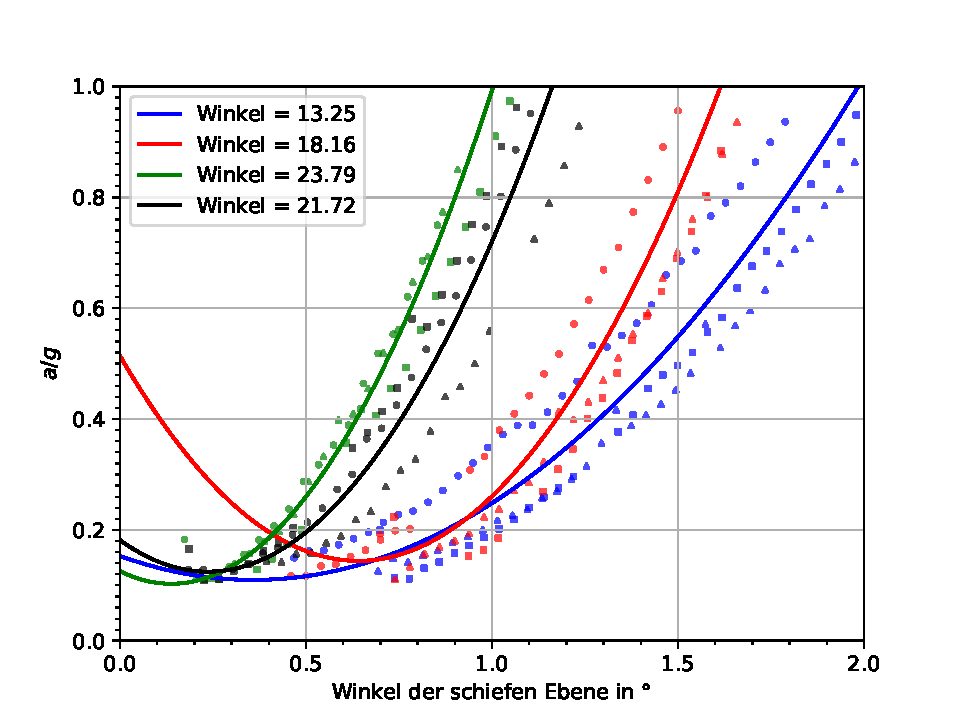
\includegraphics[width=\textwidth]{./multiple.pdf}

        \caption{Messwerte}
        \label{fig:mult}
    \end{figure}
    \begin{figure}
        \centering
        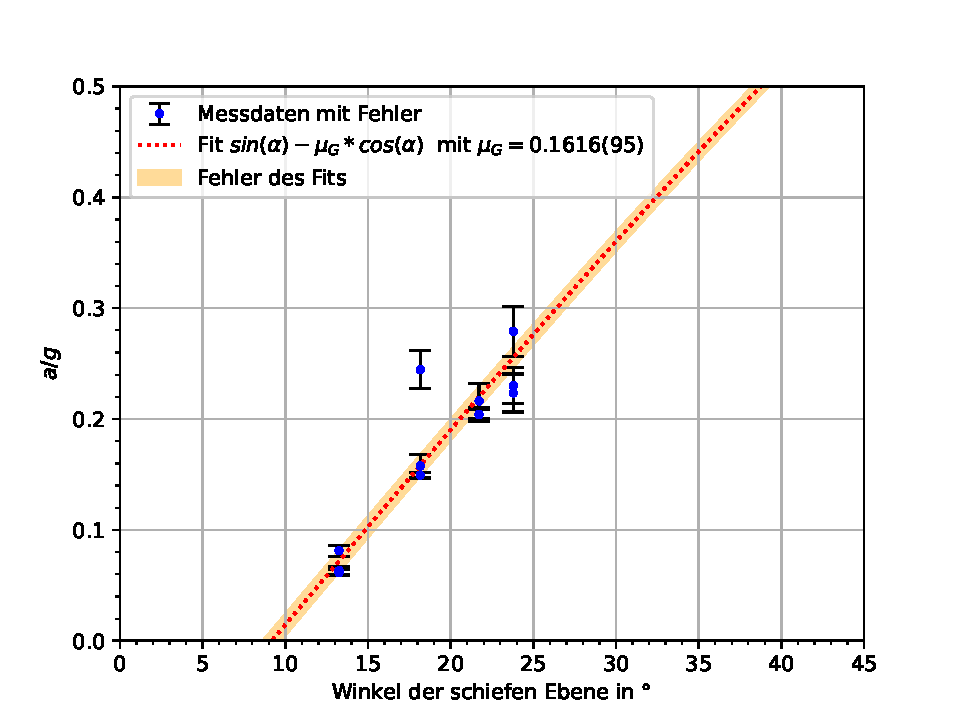
\includegraphics[width=\textwidth]{./7Plotgleit.pdf}

        \caption{Messung der Gleitreibung}
        \label{fig:Gleitr}
    \end{figure}
    Im Graphen \ref{fig:mult} werden die Messdaten und Durchschittsparabeln dargestellt. An jede Messreihe wurde 
    einzeln eine Parabel gefittet und anschießend der gewichtete Mittelwert der Parameter bestimmt, um die
    Durchschittsparabeln aufzustellen.
    Im Graph \ref{fig:Gleitr} wurden die Verhältnisse $\frac{a}{g}$ zu $\alpha$ aufgetragen. Anhand der Ausgleichkurve kann die Gleitreibung
    \begin{align}
        \mu_G = 0,1616(95)
    \end{align}
    berechnet werden. Für diesen Versuch wurden die Fehler der Winkelmessung nicht berücksichtigt, da sie viel kleiner als
    die Abweichungen der Ultraschallmessung sind. Letztere ist sehr ungenau, es entstehen manchmal Abweichungen von bis zu 20cm.
    Als Fehler wurde der Fehler des Fits der Theoriekurve von $\mu_G$ (Siehe Graph \ref{fig:Gleitr}) benutzt.


    \section{Zusammenfassung}

    Im Gegensatz zu vorangegangenen Experimenten entstanden bei diesen Versuchen sehr große Unsicherheiten. Es kann aber 
    bei jedem Experiment benannt werden, wo die Ungenauigkeiten herkommen. Auch in den Ergebnissen erkennt man diese große Ungenauigkeit.
    Ohne veränderte Versuchsaufbauten sind viel genauere Ergebnisse aber wahrscheinlich nicht zu erreichen.

    \bibliographystyle{plain}
    \bibliography{literature}

\end{document}